\documentclass{article}

\usepackage{graphicx}
\usepackage{tabularx}
\usepackage{lastpage}

\usepackage{listings}
\usepackage{xcolor}

\definecolor{mGreen}{rgb}{0,0.6,0}
\definecolor{mGray}{rgb}{0.5,0.5,0.5}
\definecolor{mPurple}{rgb}{0.58,0,0.82}
\definecolor{backgroundColour}{rgb}{0.95,0.95,0.92}

\lstdefinestyle{CStyle}{
    backgroundcolor=\color{backgroundColour},   
    commentstyle=\color{mGreen},
    keywordstyle=\color{magenta},
    numberstyle=\tiny\color{mGray},
    stringstyle=\color{mPurple},
    basicstyle=\footnotesize,
    breakatwhitespace=false,         
    breaklines=true,                 
    captionpos=b,                    
    keepspaces=true,                 
    numbers=left,                    
    numbersep=5pt,                  
    showspaces=false,                
    showstringspaces=false,
    showtabs=false,                  
    tabsize=2,
    language=C
}

\date{}
\author{Distint Howie \\ Robert Krency \\ Anthony Stepich}
\title{Lab 3}

% Geometry 
\usepackage{geometry}
\geometry{letterpaper, left=20mm, top=20mm, right=20mm, bottom=20mm}

% Fancy Header
\usepackage{fancyhdr}
\fancypagestyle{plain}{
    \fancyhf{}
    \lhead{CET 440}
    \chead{Lab3}
    \rhead{Howie - Krency - Stepich}
    \cfoot{Page \thepage \hspace{1pt} of \pageref{LastPage}}
}
\pagestyle{plain}

% Add vertical spacing to tables
\renewcommand{\arraystretch}{1.4}

% Document
\begin{document}

\maketitle

To compile, run the \textbf{make} command with the accompanying Makefile.

\begin{center}
    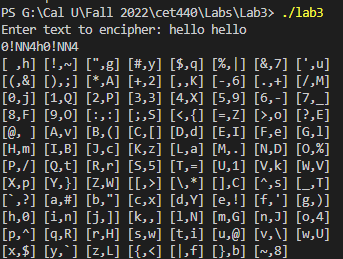
\includegraphics{screenshot.png}    
\end{center}

\subsection*{cipher.h}

\begin{lstlisting}[style=CStyle]
int * getCipher(); 
void encipher(char* input, int* cipher);
void printCipher(int* cipher);
\end{lstlisting}


\subsection*{cipher.c}

\begin{lstlisting}[style=CStyle]
\\ Initializes and scrambles a Cipher
int * getCipher(); 

\\ Enciphers the input text inplace using the given cipher
void encipher(char* input, int* cipher);

\\ Prints the cipher key to console
void printCipher(int* cipher);
\end{lstlisting}


\subsection*{lab3.c}
\begin{lstlisting}[style=CStyle]
void main();
\\ Utilizes getCipher() from cipher.c to acquire a randomized substitution cipher key
\\ Utilizes encipher() from cipher.c to encipher input text from the user
\\ Utilizes printCipher() to print the cipher key to the console
\end{lstlisting}

\pagebreak
\subsection*{Contributions}

\begin{tabular}{l l}
    Distint Howie & Input Logic, Cipher Logic, Testing \\
    Robert Krency & Cipher Logic, Testing, Accompanying Documentation \\
    Anthony Stepich & Input Logic, Cipher Logic, Testing
\end{tabular}

\end{document}